\section{Experimental Methods}\label{sec:methods}
% \begin{enumerate}
% \item \cmark  Experimental methods: (how we collect the %time series and what the times series areThis should be HPM %PAPI, which programs we model
%\item \cmark program descriptions and relevant citations
%\subitem \cmark description of \col
%\subitem \cmark description of \gcc
%\subitem \cmark description of \svd 
%\subitem \cmark description of svd regimes
% \end{enumerate}


% \subsection{Time Series Collection}

For the purposes of this study, we required a broad array of
time-series datasets from across the complexity spectrum.  We chose to
study sensor data from a computer-performance experiment.  While this
is not a common laboratory experiment, it is a highly appropriate
choice here.  Computers are extremely complicated systems and their
dynamics is surprisingly rich.
% Modern microprocessor chips contain multiple processing units and
% multi-layer memories, for instance, and they use complicated
% hardware/software strategies to maximize performance by moving data
% and threads of computation across those resources.  As a result, the
The processor and memory loads during the execution of even a very
simple program can exhibit dynamical chaos, for
instance~\cite{mytkowicz09}.  Figure~\ref{fig:col-ipc} shows an
example: a short segment of a performance trace of a four-line C
program that repeatedly initializes the upper triangle of a matrix in
column-major order.
%
 \begin{figure}[htp]
    \centering
    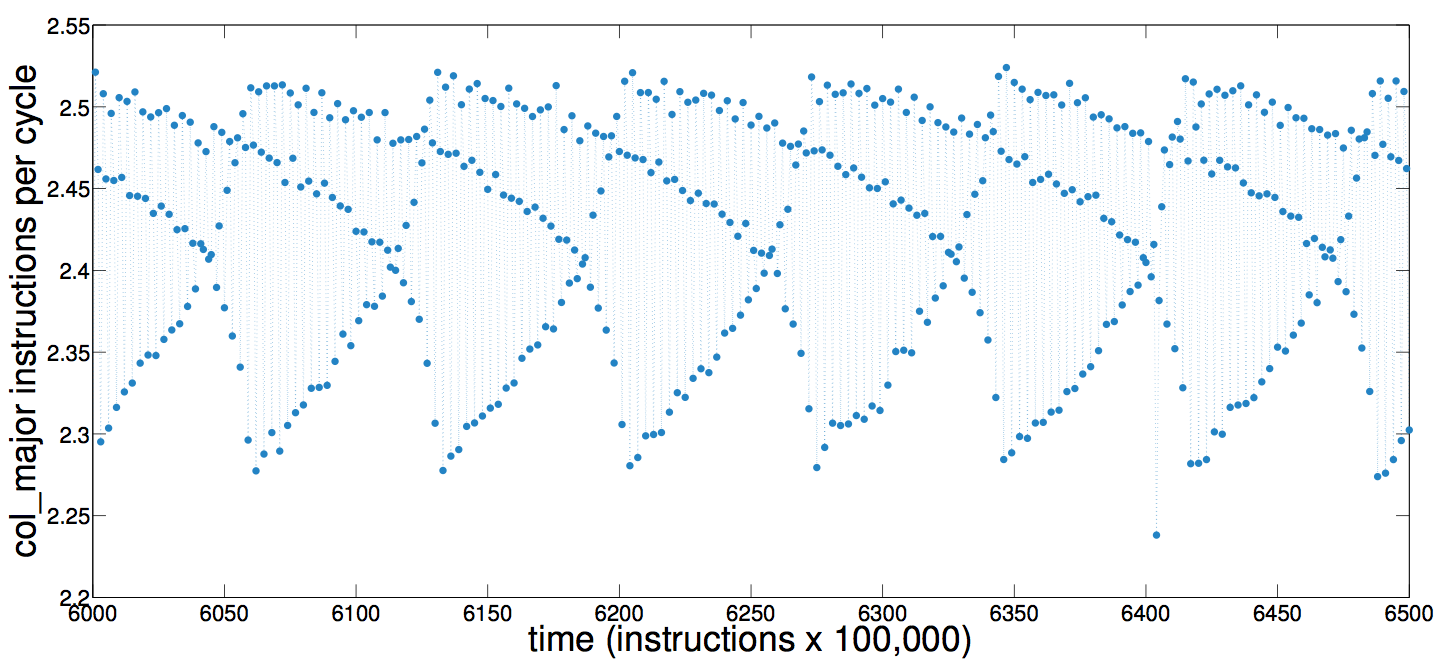
\includegraphics[width=\columnwidth]{figs/colshortts}
    % where an .eps filename suffix will be assumed under latex,
    % and a .pdf suffix will be assumed for pdflatex
    \caption{A short segment of a computer performance trace: the
      instructions per CPU clock cycle (IPC) during the execution of
      \col, a simple program that repeatedly initializes a matrix in
      column-major order.  Each point is the average IPC in a 100,000
      instruction period.}
   \label{fig:col-ipc}
  \end{figure}
%
A small change in the code can cause the dynamics to bifurcate to a
periodic regime.  
% 
% Indeed, many computer performance traces exhibit
% interesting regime changes as a program moves through the different
% phases of its operation.
By running different programs on the same computer, then, we can
produce traces that span the whole range of the complexity spectrum,
from completely predictable to completely unstructured---which makes
this an ideal testbed for this study\footnote{Predicting the
  \emph{state} of a computer, of course, would amount to solving the
  halting problem.  What we are doing here is predicting computer
  \emph{performance}, which does not violate the Rice-Shapiro
  theorem~\cite{hopcroft2007}.}.
% footnote to appease the theoretician in Josh

The time-series data sets for these experiments were collected on an
Intel Core\textsuperscript{\textregistered} i7-2600-based machine.
% 
% running the 2.6.38-8 Linux kernel.  This particular microprocessor
% chip has eight processing units, a clock rate of 3.40 GHz, and a cache
% size of 8192 KB.  
% 
We gathered performance traces during the execution of three different
programs---the simple \col loop whose performance is depicted in
Figure~\ref{fig:col-ipc} and two more-complex programs: one from the
SPEC 2006CPU benchmark suite (\gcc), and one from the LAPACK linear
algebra package (\svd).  In all of these experiments, the scalar
observation $x_i$ was a measurement of the processor performance at
time $i$ during the execution of each program.
% 
% To record these measurements, we used the {\tt libpfm4} library, via
% PAPI
% % 
% % \footnote{Performance Application Programming Interface}
% % 
% 5.2~\cite{papi}, to stop program execution at 100,000-instruction
% intervals---the unit of time in this paper---and read the contents of
% the CPU's onboard hardware performance monitors\footnote{These
%   specialty registers are built into modern microprocessors for the
%   purpose of monitoring and storage of performance data.  They can be
%   programmed to measure a wide array of processor and memory metrics
%   besides the one used here.}, which we had programmed to count how
% many instructions were executed in each clock cycle (IPC).  
% 
% These traces, and the processes that generated them, are described
% briefly in the rest of this section.
% 
For statistical validation, we collected 15 performance traces from
each of the three programs.  For an in-depth description of the
experimental setup used to gather these data,
% including discussion of the implications of the sampling interval,
please see \cite{zach-IDA10,mytkowicz09,todd-phd}. \alert{should we cite the other two ida papers? not necessarily here but they are both about predicting these traces but not cited anywhere} 


% Obviously using a system to measure itself can cause
% interference--i.e, are you measuring the generating process cleanly or
% are you adding noise to the process?---but due diligence was put into
% monitoring the generating process of these time series without
% interfering with it in a significant way.


% \subsection{The Programs: [Maybe The generating processes]{\color{blue} EDITABLE}}
% We collect performance traces of processor efficiency (IPC) of three
% exemplar programs, [If we change the title of the section, add this:
%     which act as our generating processes]---a simple
% microkernel(\col) and two complex programs: one from the SPEC 2006CPU
% benchmark suite (\gcc), and one from LAPACK (\svd). In this section we
% provide a quick explanation of each program as well as an example
% performance trace (Seen in Figures
% \ref{fig:col-ts}-\ref{fig:svd-ts-colored}.

% Commented this out because the addition of the paragraph from the
% introduction seemed like it could replace it
% 
% \col is a simple C program that repeatedly initializes the upper
% triangle of a 2048 $\times$ 2048 matrix in column-major order.
% % 
% % by looping over the following three lines of code:
% % \begin{lstlisting}
% %   for(i=0;i<2048;i++)
% %   	for(j=i;j<2048;j++)
% %   		data[j][i] = 0;
% % \end{lstlisting}
% % full listing
% % #define SIZE (2048)
% % 
% % int main(int argc, char ** argv)
% % {
% %   int i, j, n;
% %   static int data[SIZE][SIZE];
% %   
% %   for(n=0;n<numInits;n++){  
% %   for(i=0;i<SIZE;i++)
% %   	for(j=i;j<SIZE;j++)
% %   		data[j][i] = 0;
% %   }
% %   return 0;
% % }
% %
% As mentioned in Section~\ref{sec:intro}, this simple program exhibits
% surprisingly complicated behavior~\cite{mytkowicz09}.  A time series
% of the processor performance during the execution of this program is
% shown in Figure~\ref{fig:col-ts}.
% \begin{figure}[htbp]
%   \centering
%     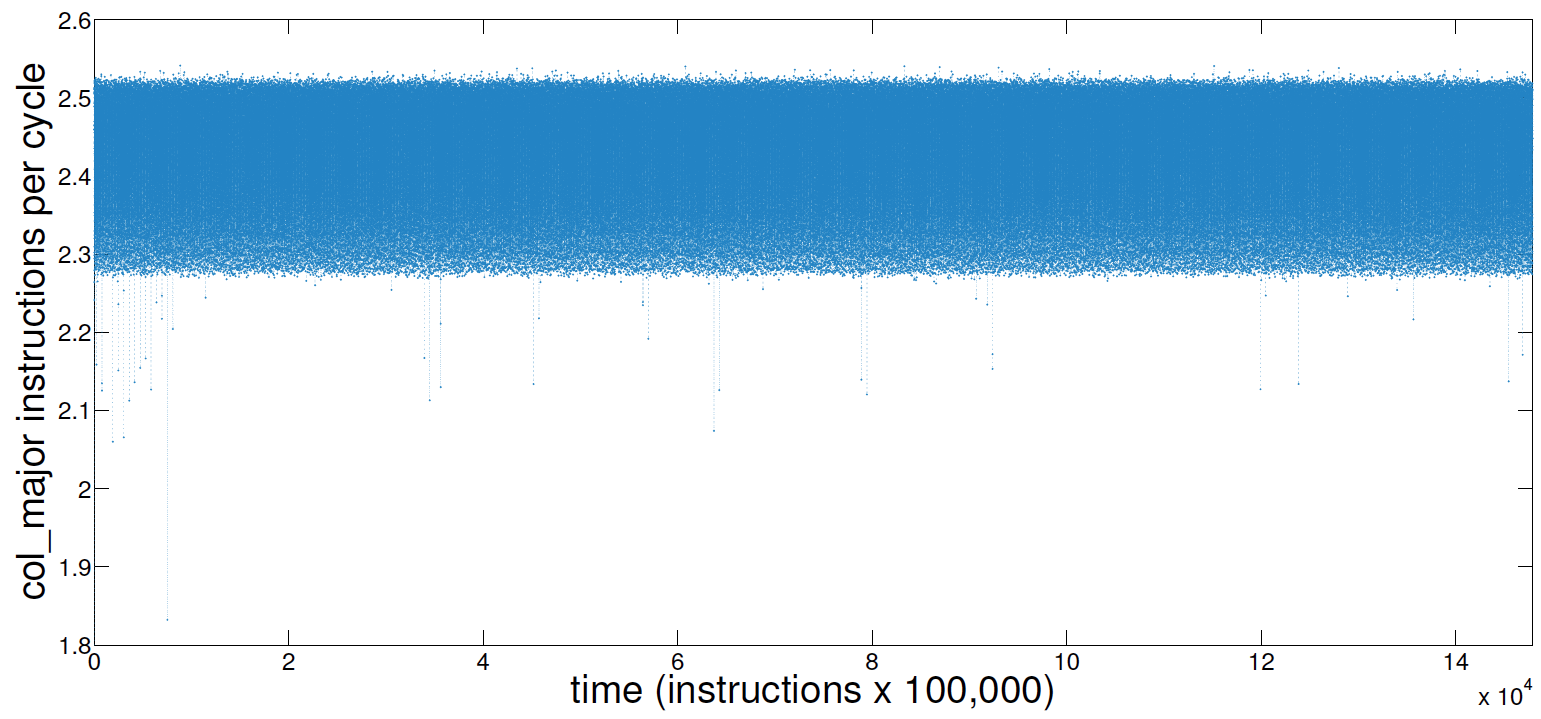
\includegraphics[width=\columnwidth]{figs/colFullTS}
%     \caption{The instructions executed per CPU clock cycle (IPC) as
%       the \col program runs.  Each point is the average IPC in a
%       100,000 instruction period. Figure~\ref{fig:col-ipc} is a
%       closeup of the first part of this signal.  }
%     \label{fig:col-ts}
%   
%   \end{figure}

The SPEC CPU2006 benchmark suite \cite{spec} is a collection of
complicated programs that are used in the computer-science community
to assess and compare the performance of different computers.  \gcc is
a member of that suite.
% 
% This program is written by Richard Stallman and is based on Version
% 3.2 of {\tt gcc}. This benchmark essentially runs as a compiler with
% many of its optimization flags enabled, compiling a series of input
% files and generating x86-64 assembly code files intended for execution
% on AMD Opteron processors\cite{spec}. 
% 
It is a \emph{compiler}: a program that translates code written in a
high-level language 
% (C, in the case of \gcc) 
into a lower-level format that can be executed by the processor chip.
Its behavior is far more complicated than that of \col, as is clear
from Figure~\ref{fig:gcc-ts}.
  \begin{figure}[t]
  \centering
    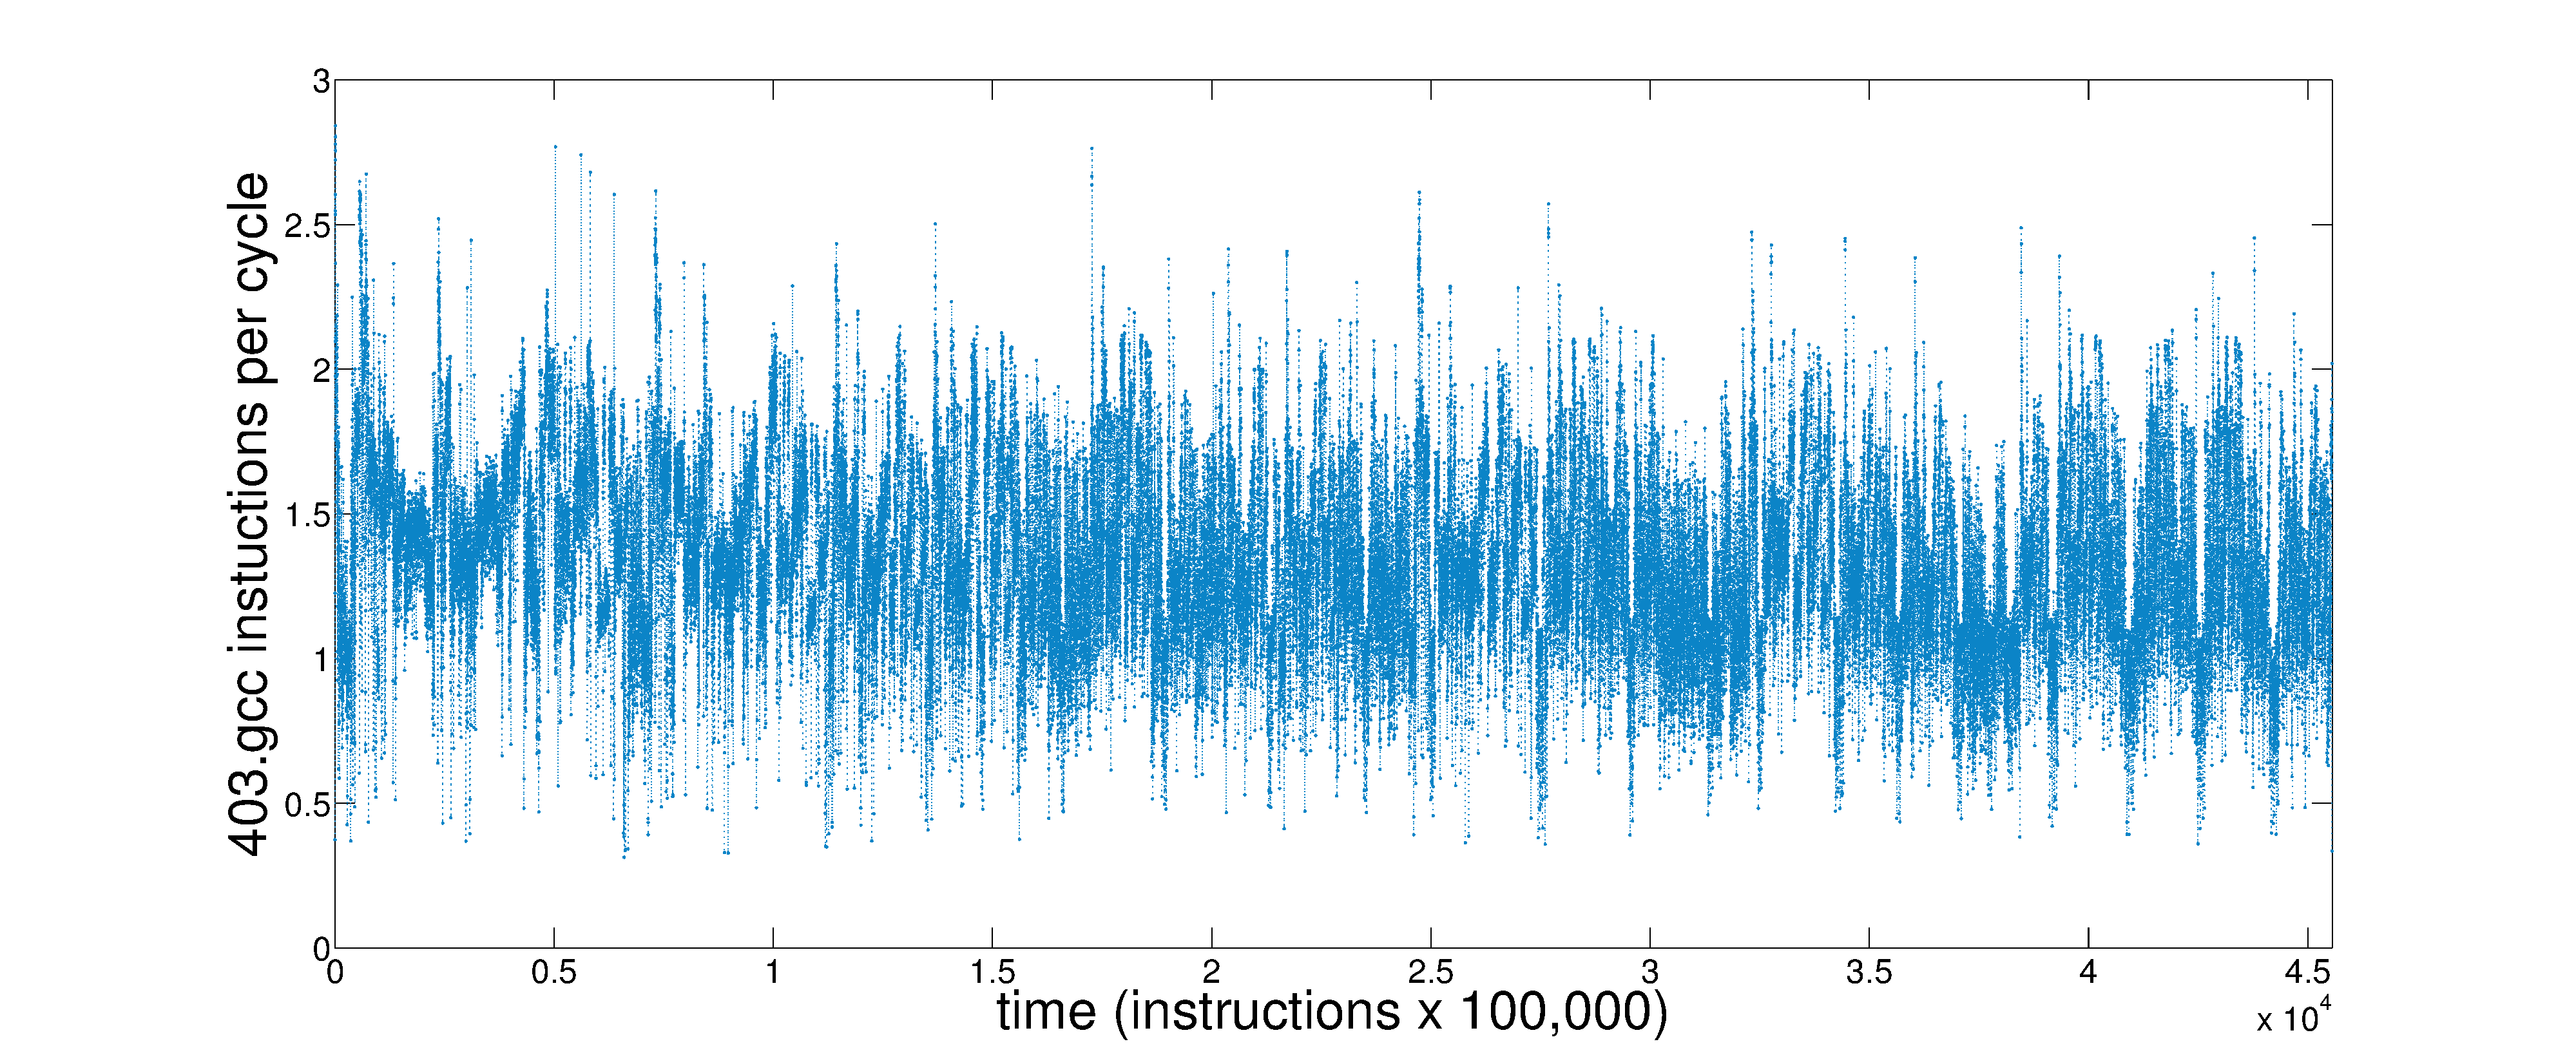
\includegraphics[width=\columnwidth]{figs/gccfullts}
    \caption{An IPC trace during the execution of \gcc.}
    \label{fig:gcc-ts}
  \end{figure}
Unlike \col, where the processor utilization is quite structured,
\gcc's performance appears almost random.

\svd is a Fortran program from the LAPACK linear algebra package
\cite{lapack}.  It calculates the singular value decomposition of a
rectangular $M$ by $N$ matrix with real-valued entries.  For our
experiments, we chose $M=750$ and $N=1000$ and generated the matrix
entries randomly.
% 
% \footnote{Multiple randomly generated matrices were
%   investigated but no measurable effect was present in the resulting
%   time series.}. 
% 
The behavior of this program as it computes the singular values of
this matrix is very interesting, as is clearly visible in Figure
\ref{fig:svd-ts-colored}.  
\begin{figure}[t]
    \centering
    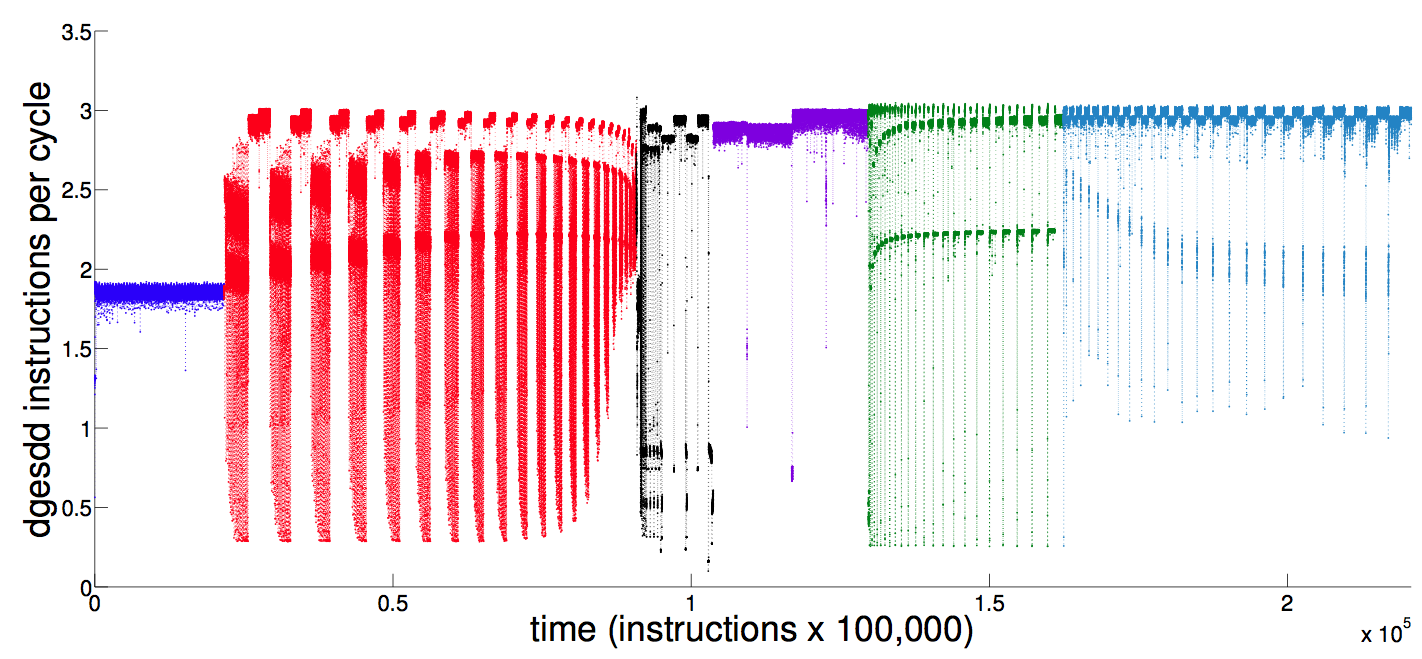
\includegraphics[width=\columnwidth]{figs/SVD1RegimesColored}
    \caption{An IPC trace during the execution of \gcc.  The colors
      identify the different \emph{segments} of the signal that are
      discussed in the text.}
    \label{fig:svd-ts-colored}
  \end{figure}
As the code moves though its different phases---diagonalizing the
matrix, computing its transpose, multiplying, etc.---the processor
utilization patterns change quite radically.  For the first
$\sim$21,000 measurements (21,000 $\times$ 100,000 instructions),
roughly 1.8 instructions are executed per cycle, on the average, by
the eight processing units on this chip.  After that, the IPC moves
through a number of different oscillatory regimes, which we have
color-coded in the figure in order to make textual cross-references
easy to track.

The wide range of behaviors in Figure~\ref{fig:svd-ts-colored}
provides a distinct advantage, for the purposes of this paper, in that
a number of different generating processes---with a wide range of
complexities---are at work in different phases of a single time
series.  The \col and \gcc traces in Figures~\ref{fig:col-ipc} and
\ref{fig:gcc-ts} appear to be far more consistent over time---probably
the result of a single generating process with consistent complexity.
\svd, in contrast, has multiple regimes, each the result of different
generating processes.  To take advantage of this, we split the signal
into six different segments, thereby obtaining an array of examples
for the analyses in the following sections.  For notational
convenience, we refer to these 90 time-series data sets\footnote{15
  runs, each with six regimes} as {\tt dgesdd$_i$}, with $i \in
\{1\dots6\}$ where $i$ corresponds to one of the six segments of the
signal, ordered from left to right.  These segments, which were
determined visually, are shown in different colors in
Figure~\ref{fig:svd-ts-colored}.  Visual decomposition is subjective,
of course, particularly since the regimes exhibit some fractal
structure.  Thus, it may be the case that more than one generating
process is at work in each of our segments.  This is a factor in the
discussion of Section~\ref{sec:results}.

%[Orphan citation?] For regimes \cite{cao2004det}
